\documentclass[letterpaper, 12pt]{article}
\usepackage{comment} % enables the use of multi-line comments (\ifx \fi) 
\usepackage{lipsum} %This package just generates Lorem Ipsum filler text. 
\usepackage{graphicx}
\usepackage{fullpage} % changes the margin
\usepackage{natbib}
\usepackage{hyperref}
\usepackage{parskip}
\usepackage{pgf}
\usepackage{amsmath}
\usepackage{amsfonts}
\usepackage{tikz}
\usepackage[margin=1in]{geometry}

\bibliographystyle{abbrvnat}
\setcitestyle{authoryear,open={(},close={)}}

\begin{document}
\counterwithin{figure}{section}

\large\textbf{Homework 4: Information} \\  
\normalsize Active Learning for Robotics (ME 455), Spring 2023, Northwestern University.
\\ \\
\normalsize\textbf{Klemens Iten}, \href{mailto:KlemensIten2023@u.northwestern.edu}{KlemensIten2023@u.northwestern.edu}\\
\normalsize   Due Mon May 29, 2023 11:59pm

\section{Ergodic Control}
% !TEX root = ./main.tex
Lorem ipsum dolor sit amet.
\clearpage
\section{Infotaxis}
% !TEX root = ./main.tex
\begin{figure}[h]
    \centering
    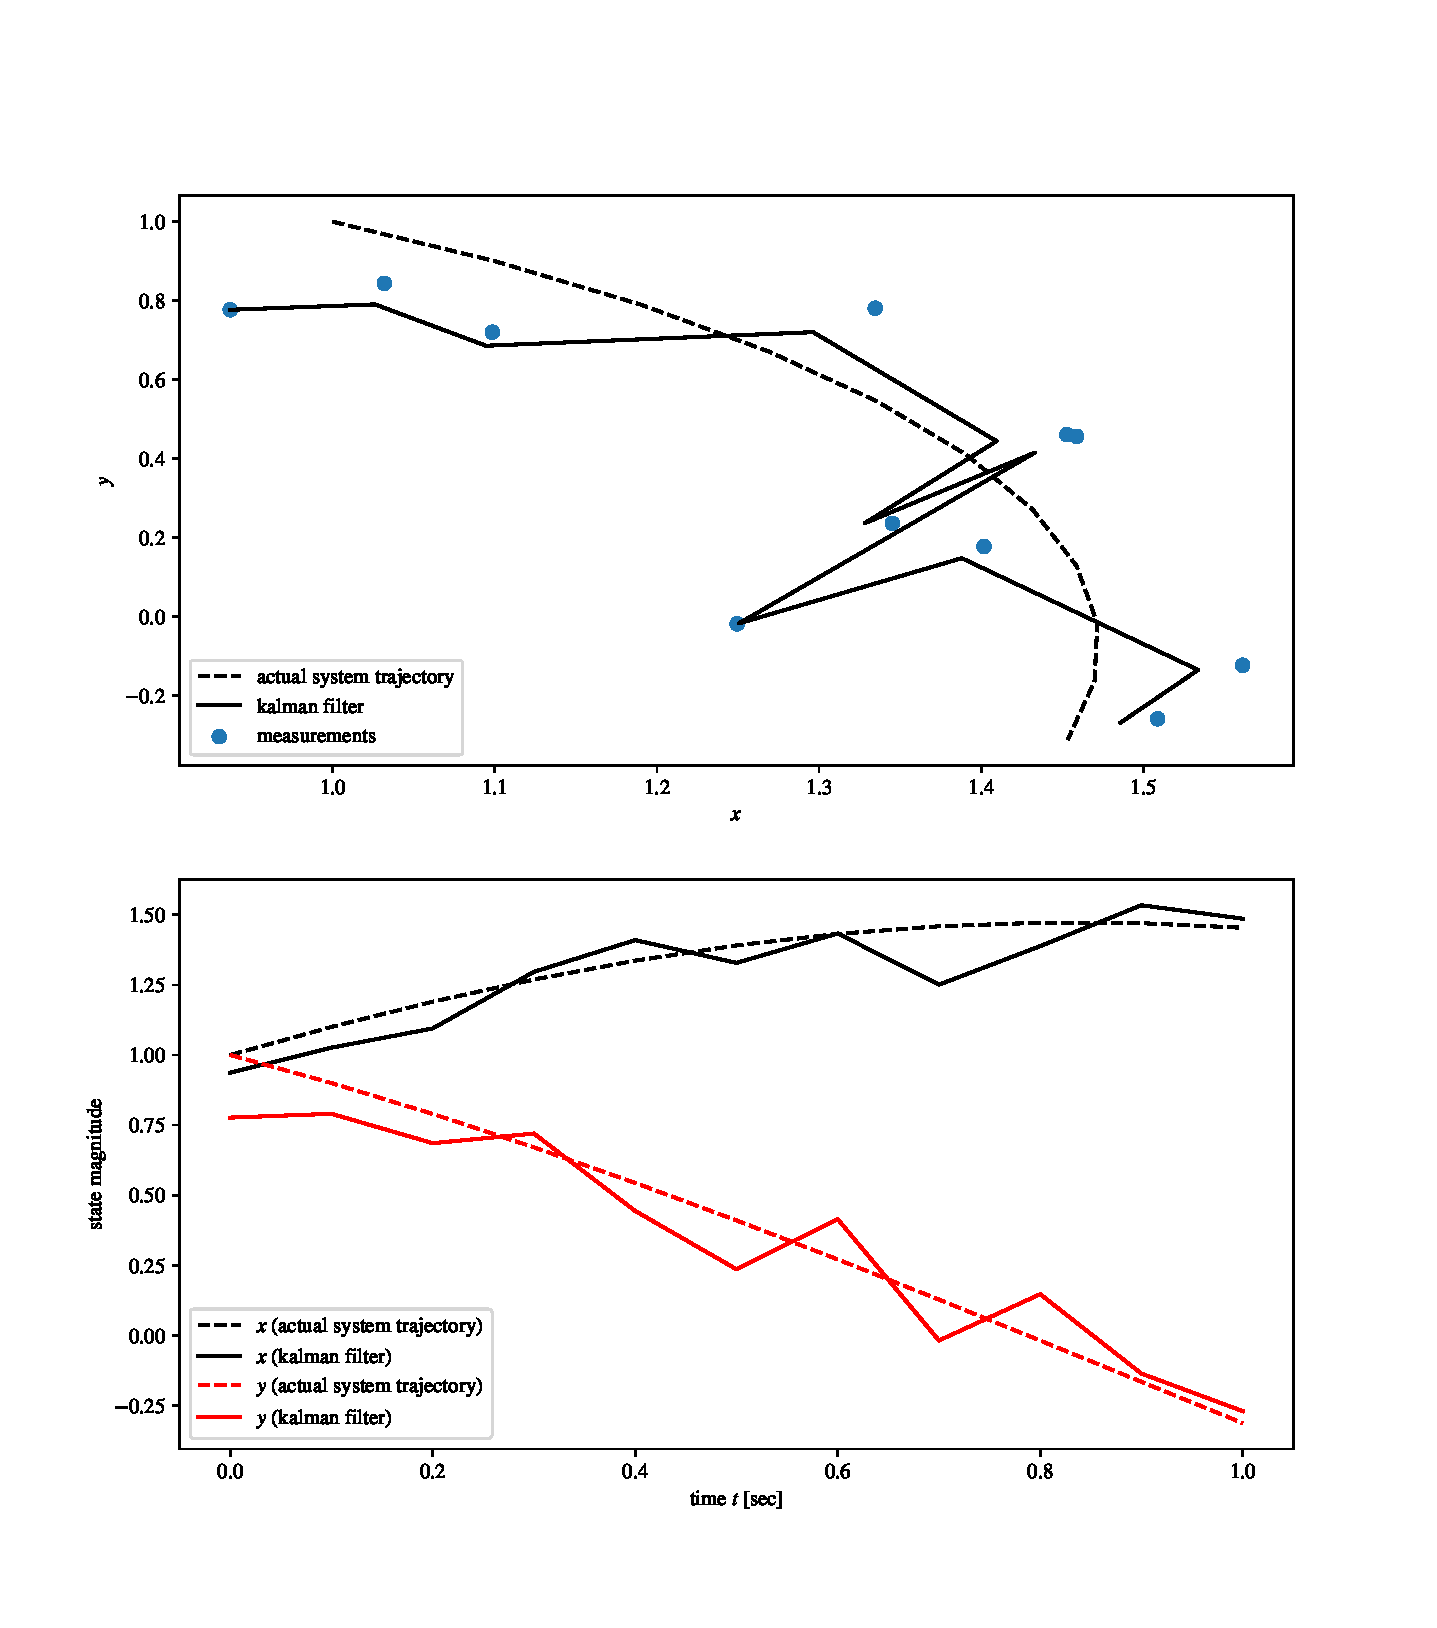
\includegraphics[width=0.88\textwidth]{q2_4.pdf}
    \vspace{-5mm}
    \caption{State evolution given measurements subject to normally distributed process and measurement noise with variance of $0.1$. 
    The nominal state evolution starting from initial condition $[1,1], dt=0.1$ is shown dashed. The filter state evolution is initialized at the first measurement with uncertainty (covariance of 0.1).}
    \label{fig:kalman}
\end{figure}
\clearpage
In figure \ref{fig:kalman}, we can see in the upper plot that the filtered trajectory apparently ``jumps'' around the map. 
This is due to the large measurement errors (variance of $0.1 \approx$ standard deviation of $0.3$ -- while our entire map only has size $0.5$ by $1$!). 
However, in the lower plot, we can see that the filter does in fact keep our filtered state roughly in the same region as the nominal system trajectory. 

The filtered state has the following covariances:

\begin{center}
    \begin{tabular}{ |p{2.5cm}||p{2.5cm}|p{4cm}|p{4cm}|  }
        \hline
        \multicolumn{4}{|c|}{Updated (a posteriori) estimate covariance} \\
        \multicolumn{4}{|c|}{$P_{k\mid k} = \begin{bmatrix}
            \textsc{Cov}(x,x) & \textsc{Cov}(x,y) \\
            \textsc{Cov}(y,x) & \textsc{Cov}(y,y)
            \end{bmatrix} $}\\
        \multicolumn{4}{|c|}{with $\textsc{Cov}(x,y)=\textsc{Cov}(y,x)=0$}\\

        \hline
        Measurement& $t$ (sec) & \textsc{Cov}($x,x$) & \textsc{Cov}($y,y$) \\
        \hline
        1   & 0.0  & 0.1 & 0.1 \\
        2  & 0.1   & 0.06677740 & 0.06677740 \\
        3 & 0.2    & 0.07518671 & 0.07518671 \\
        4  & 0.3   & 0.08023872 & 0.08023872 \\
        5 & 0.4    & 0.08360925 & 0.08360925 \\
        6 & 0.5    & 0.08601793 & 0.08601792 \\
        7 &  0.6   & 0.08782497 & 0.08782497 \\
        8 &  0.7   & 0.08923071 & 0.08923071 \\
        9 &  0.8   & 0.09035542 & 0.09035542 \\
        10 & 0.9   & 0.09127568 & 0.09127568 \\
        11 & 1.0   & 0.09204254 & 0.09204254 \\
        \hline  
       \end{tabular}  
\end{center}

We can see that the covariance is a diagonal matrix (since measurements of $x$ and $y$ are independent random variables) initialized at our state/sensor noise variance of $0.1$. 

This initial covariance gets reduced (no filtering for the first step since we initialize our filter at the first uncertain measurement), 
but thanks to the Kalman filter we can reduce the covariance below $0.1$. The covariance grows in magnitude (additive noise over time) and presumably approaches $0.1$ gradually.

%=============================================
% \bibliographystyle{}
% \small
% \bibliography{Cites.bib}

\end{document}

\ifx
Comments!
\fi

% ===========

\ifx

%==============
